\documentclass{report}
\usepackage{setspace}
\usepackage{contour}
\usepackage{ulem}
\usepackage{caption}
\usepackage{subcaption}
\usepackage{geometry}
\usepackage{multicol}
\usepackage{array,etoolbox}
\usepackage{fancyhdr}
\usepackage[toc,page]{appendix}
\geometry{
letterpaper,
left=1in,
right=1in,
bottom=1in,
top=1in,
}

\pagestyle{fancy}
\lhead{PeaPod - Design Brief}
\rhead{UTAG}

\newcounter{metricnumber}
\setcounter{metricnumber}{0}
\newcommand\rownumber{\stepcounter{metricnumber}\arabic{metricnumber}}

\renewcommand{\ULdepth}{1.5pt}
\contourlength{0.8pt}

\newcommand{\myuline}[1]{%
  \uline{\phantom{#1}}%
  \llap{\contour{white}{#1}}%
}

% \renewcommand{\baselinestretch}{1.5}
\setstretch{1.5}

\begin{document}

\begin{titlepage}
    \begin{center}
        \vspace*{1.2cm}
        
        \textbf{\large{PeaPod - Design Brief}}
        
        \vspace{0.5cm}
        Submission to the NASA/CSA Deep Space Food Challenge

        \vfill
        
        Jayden Lefebvre - Lead Engineer\\\small{jayden.lefebvre@mail.utoronto.ca}
        
        \vspace{2.5cm}
        
        Revision 0.2\\
        University of Toronto Agritech\\
        May 5th, 2021
        
    \end{center}
 \end{titlepage}

\thispagestyle{plain}

\tableofcontents
\newpage

\section{Introduction}
\label{sec:intro}

\subsection{Purpose}
\label{sec:purpose}

The purpose of this design brief is to outline the requirements for a submission 
to the NASA/CSA Deep Space Food Challenge Phase 1 \cite{dsfc}. In doing so, it also
documents the scope of a design submitted by University of Toronto Agritech (UTAG).

The goal of the Deep Space Food Challenge is for participants to "Create novel 
food production technologies or systems that require \myuline{minimal inputs} and 
\myuline{maximize safe, nutritious, and palatable food outputs} for 
\myuline{long-duration space missions}, and which have potential to benefit 
people on Earth." \cite{applicantguide}

\subsection{Framing Structure}
\label{sec:structure}

This document achieves its purpose via "top-down" framing (Section \ref{sec:framing}), with each subsection's 
entries being derived from the entries of the previous\footnote{Each objective and metric has 
a numbered reference to the entry it was derived from (\myuline{\textbf{S}}takeholder 
\myuline{\textbf{1}} : S1, \myuline{\textbf{H}}igh-\myuline{\textbf{L}}evel Objective 
\myuline{\textbf{8}} : HL8, etc.)}.

\begin{itemize}
    \item \textbf{\ref{sec:opportunity} - Opportunity}: A succinct scoped challenge 
    statement.
    \item \textbf{\ref{sec:requirements} - Requirements}: Categorical or scoping constraints.
    \item \textbf{\ref{sec:stakeholders} - Stakeholders}: Persons and groups in 
    consideration.
    \item \textbf{\ref{sec:hlos} - High-Level Objectives}: Conceptual aims, DfX; derived 
    from Requirements and Stakeholders.
    \item \textbf{\ref{sec:llos} - Low-Level Objectives}: Tactical goals; derived from HLOs.
    \item \textbf{\ref{sec:metrics} - Metrics}: Quantitative measures of design success, fit, 
    utility, etc; derived from LLOs.
\end{itemize}

\newpage

\subsection{Scope and Justification}
\label{sec:scope}

Phase 1 development, testing, and assessment is scoped to terrestrial/Earth-like operational constraints \cite{applicantguide}:
\begin{itemize}
    \item Gravity (9.81 m/s${}^2$);
    \item Ambient atmospheric pressure (101,325 Pa);
    \item Ambient atmospheric/"room" temperature (22 °C);
    \item Ambient atmospheric humidity (50 \%RH);
\end{itemize}

In addition, it is important to note that the solution "need not meet the full nutritional requirements of 
future crews, but can contribute significantly to, and integrate with, a comprehensive food system." \cite{applicantguide}

The three underlined criteria in the challenge statement in Section \ref{sec:purpose} have also helped to define the 
scope of this brief:

\begin{enumerate}
\item The longer the duration of the space mission (up to and including interplanetary 
    travel and permanent colonization) the lesser the feasability of resupply
    \footnote{Minimal resupply is also listed as a constraint directly in the challenge 
    details \cite{applicantguide}.}.
\item The lesser the feasability of resupply, and the more minimal the input 
    (i.e. launch mass), the more the design will need to generate net-new food 
    grown on-board during the mission \footnote{Any other food production technologies 
    would be taking advantage of existing food; as such this is the basis for the 
    problem.}.
\item The minimization of inputs (launch mass), the minimization of other negative 
    criteria such as growth time, design complexity, etc. and the maximization of 
    safety (pathogenic and otherwise) means that food animal growth has been deemed 
    not feasible, and is outside the scope of this brief. Thus, the design should 
    focus on food-producing plant (or crop) growth\footnote{This is primarily an 
    issue in-transit; for colonization, non-plant food production systems should 
    definitely be considered.}.
\item Spacecraft are not good crop growth systems (lack of water access, proper 
    lighting and nutrition, etc.), thus the design should encompass a crop growth 
    environment that:
    \begin{enumerate}
        \item provides of all necessary crop growth inputs (water, nutrients, lighting, 
        etc.)
        \item contains or otherwise encompasses a viable crop growth environment 
        (temperature, humidity, gas concentrations, airflow, etc.)
        \item has control over all parameters of both a) and b) (environment parameters); 
        these together are the (crop growth) environment conditions.
    \end{enumerate}
\item To maximise safety (of both the crops and the crew) and redundancy, and to minimize 
    inputs (required human interaction), the environment should be automated and isolated 
    from the spacecraft cabin with regards to all environment conditions (thermally, 
    water-tight, etc.) unless beneficial and efficient (i.e no loss).

% \end{enumerate}
% \newpage
% \large
% \textbf{1.3 \ \ \ Scope and Justification (Cont'd)}
% \normalsize
% \begin{enumerate}

\item A greater degree of nutrition and palatability of food outputs implies a greater 
    variety of crops (incl. leafy greens, fruits/fruiting vegetables, root vegetables, 
    algaes, etc.); as such the food production system should be able to generate a 
    continuous variety of environmental conditions such that any number of food crops 
    could be grown within.
\item The demand for high crop variety, automation, parameter control, etc. implies 
    the use of a hydroponic/aeroponic/hybrid crop growth method.
\end{enumerate}

\subsection{Definitions}
\label{sec:definitions}
A number of useful definitions have emerged from the above scoping:

\begin{enumerate}
\item (Crop Growth) Environment - The environment within which the crop grows/with which 
the crop interacts; the environment parameters in terms of their relationship with the 
crop and its growth.
\item (Crop Growth) Environment Parameters - The (often quantitative) parameters of the 
crop environment, as well as any and all other parameters relevant to crop growth.
\item Crop Growth System - Includes the physical enclosure (containing the crops and the 
controlled environment; incl. isolation) as well as any infrastructure required to 
generate the crop growth environment and control all environment conditions; satisfies 
all requirements of this brief.
\end{enumerate}

\newpage

\section{Framing}
\label{sec:framing}

\subsection{Opportunity}
\label{sec:opportunity}

Design a fully automated and isolated hydroponic/aeroponic crop growth system for the 
Deep Space Food Challenge Phase 1\cite{dsfc}, able to generate any environment from a 
combination of independent environment parameters.

\subsection{Requirements}
\label{sec:requirements}

Compiled from DSFC Applicant Guide details \cite{applicantguide} and an excerpt of NASA-STD-3001: Section 7.1 Food and Nutrition\footnote{Additional nutrition and caloric output constraints relative to activity level, crew details, etc. are provided; however they are not in direct consideration as of Phase 1.} \cite{nutrition}:
\begin{enumerate}
    \item \textit{Helps} fill food gaps for a \textbf{three-year} round-trip mission with 
    \textbf{no resupply}:
    \begin{enumerate}
        \item Feeds a crew of \textbf{four (4)} people;
        \item Provides the capability to maintain food safety and nutrition \textbf{during all phases} of the mission;
        \item Provides food that is \textit{acceptable} to the crew \textbf{for the duration} of the mission;
        \item Produces \textbf{varied, safe, nutritious, and palatable} food outputs that 
        can provide \textbf{all 
        daily nutritional needs} and require \textbf{little processing time}\footnote{It is 
        assumed that fresh (or packaged unprepared) edible plant products are already 
        prepared on existing space missions, and that this preparation meets this requirement; 
        thus, preparation time is outside the scope of this design brief.} for crew members;
    \end{enumerate}
    \item Improve the accessibility of food on Earth; in particular, via production 
    directly in urban centres and in remote and harsh environments:
    \begin{enumerate}
        \item Enhance local production;
        \item Reduce food supply chain shortages;
        \item Reduce the impact on the resources needed for food production;
        \item Able to operate in harsh and remote environments;
    \end{enumerate}
    \item Achieve the \textbf{greatest amount of food output} with \textbf{minimal inputs} and \textbf{minimal waste};
    \item Transmits \textbf{operational data and limited video} to a remote location, and receives periodic \textbf{operational commands}.
\end{enumerate}

% \newpage
% \large
% \textbf{2.2 \ \ \ Requirements (Cont'd)}
% \normalsize

Extracted from scoping:
\begin{enumerate}
    \setcounter{enumi}{3}
    \item Must be able to operate under Earth-like conditions (See Section \ref{sec:scope});
    % TODO: more
\end{enumerate}

\setstretch{1}

\subsection{Stakeholders}
\label{sec:stakeholders}

\begin{enumerate}
    \item Food Product Consumers
    \item NASA/CSA Stakeholders - Spacecraft feasability and optimization criteria
    \item Crops - Crop growth metrics
    % \item G7, G20, UN, and other global development entities
\end{enumerate}

\newpage

\subsection{Objectives}
\label{sec:objectives}

\begin{multicols}{2}[\subsubsection{High-Level}\label{sec:hlos}]
    \begin{enumerate}
        \item Food Output Suitability \hfill (S1, R1, R1a, R2a)
        \item Environment Control, Automation, and Optimization \hfill (S2, S3, R1b, R2c, R2d, R3)
        \item Efficiency \hfill (S1, S2, R1, R2a, R2c, R3)
        \item Cross-Contamination \hfill (S1, S2, R1c)
        \item Safety, Redundancy \hfill (S1, S2, R1b, R2b)
        \item Modularity, Repairability \hfill (S1, S2, R2d)
        \item Feasability \hfill (S2)
    \end{enumerate}
\end{multicols}

\begin{multicols}{2}[\subsubsection{Low-Level}\label{sec:llos}]
    \begin{enumerate}
        \item Output Food Variety \hfill (HL1)
        \item Output Food Palatability \hfill (HL1)
        \item Nutrient Output \hfill (HL1)
        \item Energy Output \hfill (HL1, HL4)
        \item Air Temperature Control \hfill (HL2)
        \item Air Humidity Control \hfill (HL2)
        \item Gas Concentration Control \hfill (HL2)
        \item Lighting Control \hfill (HL2)
        \item Light Isolation \hfill (HL2)
        \item Thermal Isolation \hfill (HL2)
        \item Water-tightness \hfill (HL2, HL5)
        \item Airflow \hfill (HL2)
        \item Water Flow Rate \hfill (HL2)
        \item Water Temperature \hfill (HL2)
        \item Germination Success \hfill (HL2)
        \item High Degree of Automation \hfill (HL3)
        \item Energy Efficiency \hfill (HL3)
        \item Water Usage Efficiency \hfill (HL3)
        \item Plant Matter Usage \hfill (HL3)
        \item Gas Exchange Incentive \hfill (HL3)
        \item Number of Harvests \hfill (HL3)
        \item Time-To-Harvest/-Reharvest \hfill (HL3)
        \item Germination Time \hfill (HL3)
        \item Growth Time \hfill (HL3)
        \item Potential for Cross-Contamination \hfill (HL4)
        \item Structural Safety \hfill (HL5)
        \item Electrical/Power Safety \hfill (HL5)
        \item Power Supply Redundancy \hfill (HL5)
        \item Infrastructure Redundancy \hfill (HL5)
        \item Growth Container Modularity \hfill (HL6)
        \item Infrastructure Modularity Support \hfill (HL6)
        \item Growth Container Repairability \hfill (HL6)
        \item Infrastructure Repairability \hfill (HL6)
        \item Documentation Completion \hfill (HL6)
        \item Design Complexity \hfill (HL6)
        \item Tool Speciality and Number \hfill (HL6)
        \item Cost \hfill (HL7)
        \item Size \hfill (HL7)
    \end{enumerate}
\end{multicols}

\newpage

\subsection{Metrics}
\label{sec:metrics}

\begin{center}
    \begin{tabular}{| @{\makebox[2em][l]{\rownumber}} | l | l |} 
        \hline
        \multicolumn{1}{| @{\makebox[2em][l]{\textbf{\#}}} | l |}{\textbf{Metric}} & \textbf{Units}\\ 
        \hline
        Number of Suitable Crop Species \hfill (LL1) & \# (per crop) \\
        \hline
        Quality/Palatability of Crop Output \hfill (LL2) & 1-10 (per crop) \\
        \hline
        Crop Nutrient Concentration \hfill (LL3) & \% (per crop) \\
        \hline
        Protein Output Density \hfill (LL3) & g/kg \\
        \hline
        Protein Output \hfill (LL3) & kCal/crewmember (\%TDEI) \\
        \hline
        Carbohydrate Output \hfill (LL3) & kCal/crewmember (\%TDEI) \\
        \hline
        Lipid Output\hfill (LL3) & kCal/crewmember (\%TDEI) \\
        \hline
        $\Omega$-6 Fatty Acid Output\hfill (LL3) & g/day/crewmember \\
        \hline
        $\Omega$-3 Fatty Acid Output\hfill (LL3) & g/day/crewmember \\
        \hline
        Saturated Fat Output \hfill (LL3) & kCal/crewmember (\%TDEI) \\
        \hline
        Trans Fatty Acids Output \hfill (LL3) & kCal/crewmember (\%TDEI) \\
        \hline
        Cholesterol Output \hfill (LL3) & mg/day/crewmember \\
        \hline
        Fiber Output \hfill (LL3) & g/day/crewmember \\
        \hline
        Caloric Output per Day \hfill (LL4) & kCal/24hr \\
        \hline
        Air Temperature Control Range \hfill (LL5) & min, max °C \\
        \hline
        Air Temperature Control Rate \hfill (LL5) & °C/sec at each °C \\
        \hline
        Air Temperature Control Stability \hfill (LL5) & $\pm$°C at each °C \\
        \hline
        Air Humidity Control Range \hfill (LL6) & min, max \%RH \\
        \hline
        Air Humidity Control Rate \hfill (LL6) & \%RH/sec at each \%RH \\
        \hline
        Air Humidity Control Stability \hfill (LL6) & $\pm$\%RH at each \%RH \\
        \hline
        CO${}_2$ Concentration Control Range \hfill (LL7) & min, max ppm CO${}_2$ \\
        \hline
        CO${}_2$ Concentration Control Rate \hfill (LL7) & ppm CO${}_2$/sec at each ppm 
        CO${}_2$ \\
        \hline
        CO${}_2$ Concentration Control Stability \hfill (LL7) & $\pm$ppm CO${}_2$ at 
        each ppm CO${}_2$ \\
        \hline
        O${}_2$ Concentration Control Range \hfill (LL7) & min, max ppm O${}_2$ \\
        \hline
        O${}_2$ Concentration Control Rate \hfill (LL7) & ppm O${}_2$/sec at each ppm 
        O${}_2$  \\
        \hline
        O${}_2$ Concentration Control Stability \hfill (LL7) & $\pm$ppm O${}_2$ at each 
        ppm O${}_2$ \\
        \hline
        Light Spectrum Wavelength Control Range \hfill (LL8) & min, max nm \\
        \hline
        Light Spectrum PAR Match \hfill (LL8) & \% (each crop) \\
        \hline
        Light Spectrum Intensity Control Range \hfill (LL8) & min, max $\mu$mol 
        m${}^{-2}$sec${}^{-1}$ at each nm \\
        \hline
        Light Spectrum Intensity Control Stability \hfill (LL8) & $\pm\mu$mol 
        m${}^{-2}$sec${}^{-1}$ at each nm \\
        \hline
        Light Captured by Non-Photosynthetic Surfaces \hfill (LL9) & \% \\
        \hline
        Outside Light Penetration \hfill (LL9) & \% \\
        \hline
        Heat Transfer \hfill (LL10) & $\pm$W at each °C \\
        \hline
        Water Loss due to Leaks, Evaporation \hfill (LL11) & mL/hr \\
        \hline
        Internal Circulation Airflow Control Range \hfill (LL12) & min, max m${}^3$/min \\
        \hline
        Gas Exchange due to Leaks \hfill (LL12) & m${}^3$/min \\
        \hline
        Maximum Intentional Gas Exchange \hfill (LL12) & m${}^3$/min \\
        \hline
        Nutrient Solution Delivery Rate Control Range \hfill (LL13) & min, max 
        mL/plant/sec \\
        \hline
        Nutrient Solution Delivery Rate Control Rate \hfill (LL13) & mL/plant/sec${}^2$ at each mL/plant/sec  \\
        \hline
        Nutrient Solution Delivery Rate Control Stability \hfill (LL13) & 
        $\pm$mL/sec/plant at each mL/sec/plant \\
        \hline
   \end{tabular}
\end{center}
\newpage

\textbf{\large{2.5 \ \ Metrics (Cont'd)}}
\normalsize

\begin{center}
    \begin{tabular}{| @{\makebox[2em][l]{\rownumber}} | l | l |} 
        \hline
        \multicolumn{1}{| @{\makebox[2em][l]{\textbf{\#}}} | l |}{\textbf{Metric}} & \textbf{Units}\\ 
        \hline
        Nutrient Solution Temperature Control Range \hfill (LL14) & min, max °C \\
        \hline
        Nutrient Solution Temperature Control Rate \hfill (LL14) & °C/sec at each °C  \\
        \hline
        Nutrient Solution Temperature Control Stability \hfill (LL14) & 
        $\pm$°C at each °C  \\
        \hline
        Germination Success Rate \hfill (LL15) & \% \\
        \hline
        Required Human Intervention Time - Maintenance \hfill (LL16) & hrs/week \\
        \hline
        Required Human Intervention Time - Setup \hfill (LL16) & hrs \\
        \hline
        Energy Efficiency - In (Power) vs. Out (kCal + Loss) \hfill (LL17) & \% \\
        \hline
        Necessary Water Waste per Day \hfill (LL18) & L/day \\
        \hline
        Water Recycling from Spacecraft Systems \hfill (LL18) & L/day \\
        \hline
        Initial Water Requirement \hfill (LL18) & L \\
        \hline
        Plant Matter Usage \hfill (LL19) & \% \\
        \hline
        CO${}_2$ Capture - Fraction of Typical Reclaimer Consumption \hfill (LL20) & \% \\
        \hline
        O${}_2$ Production - Fraction of Typical Reclaimer Production \hfill (LL20) & \% \\
        \hline
        Number of Harvests per Planting \hfill (LL21) & \# (each crop)\\
        \hline
        Harvest to Reharvest - Fruiting Crops \hfill (LL22) & min (each crop)  \\
        \hline
        Seedling to Harvest \hfill (LL22, LL24) & min (each crop) \\
        \hline
        Germination Time \hfill (LL23) & min (each crop) \\
        \hline
        Potential for Cross-Contamination - Germination \hfill (LL25) & \% (each event)\\
        \hline
        Potential for Cross-Contamination - Planting \hfill (LL25) & \% (each event)\\
        \hline
        Potential for Cross-Contamination - Harvest \hfill (LL25) & \% (each event)\\
        \hline
        Factor of Safety \hfill (LL26) & FOS (each structure)\\
        \hline
        Mounting Stability - System to Surroundings \hfill (LL26) & FOS (each mount) \\
        \hline
        Mounting Stability - Infrastructure to System \hfill (LL26) & FOS (each mount) \\
        \hline
        Risk of Electrical Malfunction \hfill (LL27) & \% \\
        \hline
        Backup Power Systems? \hfill (LL28) & Y/N \\
        \hline
        Incremental Power-On? \hfill (LL28) & Y/N \\
        \hline
        Backup Water Systems? \hfill (LL29) & Y/N \\
        \hline
        Infrastructure Failure Notification? \hfill (LL29) & Y/N \\
        \hline
        Independent Crop Growth Environments? \hfill (LL30) & Y/N \\
        \hline
        Support for N+1 Crop Growth Environments? \hfill (LL31) & Y/N \\
        \hline
        Lighting System Swappable? \hfill (LL32) & Y/N \\
        \hline
        Heating/Cooling System(s) Swappable? \hfill (LL32) & Y/N \\
        \hline
        Water Delivery System(s) Swappable? \hfill (LL32) & Y/N \\
        \hline
        Lighting System Swappable? \hfill (LL32) & Y/N \\
        \hline
        Computer Subsystems Swappable? \hfill (LL33) & Y/N \\
        \hline
        All Fabrication Procedures, Tools, and Materials Documented? \hfill (LL34) & Y/N \\
        \hline
        All Assembly Procedures, Tools, and Materials Documented? \hfill (LL34) & Y/N \\
        \hline
        All Repair Procedures, Tools, and Materials Documented? \hfill (LL34) & Y/N \\
        \hline
        Total Fabrication, Assembly, and Startup Time \hfill (LL35) & min \\
        \hline
        Total Number of Tools Required \hfill (LL36) & \# \\
        \hline
    \end{tabular}
\end{center}

\newpage

\textbf{\large{2.5 \ \ Metrics (Cont'd)}}
\normalsize

\begin{center}
    \begin{tabular}{| @{\makebox[2em][l]{\rownumber}} | p{11.5cm} | p{3.2cm} |} 
        \hline
        \multicolumn{1}{| @{\makebox[2em][l]{\textbf{\#}}} | l |}{\textbf{Metric}} & \textbf{Units}\\ 
        \hline
        Number of New Tools Required \hfill (LL36) & \# \\
        \hline
        Cost \hfill (LL37) & CAD \\
        \hline
        Outer Dimensions \hfill (LL38) & m (W, D, H) \\
        \hline
        Outer Volume \hfill (LL38) & m${}^3$ \\
        \hline
        Power Consumption \hfill (LL38) & W \\
        \hline
        Mass \hfill (LL38) & kg \\
        \hline
    \end{tabular}
\end{center}

\subsection{Constraints}
\begin{center}
    \begin{tabular}{|l|p{12.6cm}|p{1.3cm}|}
        \hline
        \textbf{Metric} & \textbf{Constraint} & \textbf{Source} \\
        \hline
        M45 & 4 hrs/week & \cite{applicantguide}\\
        \hline
        M83 & Fits through 1.07m x 1.90m doorway; W<1.829m, D<2.438m, H<2.591m & \cite{applicantguide} \\
        \hline
        M84 & $\le$ 2 m${}^3$ & \cite{applicantguide}\\
        \hline
        M85 & Avg. <1500W; Peak < 3000W & \cite{applicantguide}\\
        \hline
    \end{tabular}
\end{center}

\subsection{Criteria}
\begin{center}
    \begin{tabular}{|l|p{12.6cm}|p{1.3cm}|}
        \hline
        \textbf{Metric} & \textbf{Criteria; Reason} & \textbf{Source} \\
        \hline
        M34 & Minimize; Reduce System Inputs & \cite{applicantguide} \\
        \hline
        M48 & Minimize; Reduce System Inputs & \cite{applicantguide} \\
        \hline
        M49 & Maximize; Reduce System Inputs & \cite{applicantguide} \\
        \hline
        M50 & Minimize; Reduce System Inputs & \cite{applicantguide} \\
        \hline
        M86 & Minimize; Reduce System Inputs & \cite{applicantguide} \\
        \hline
    \end{tabular}
\end{center}

Refer to Appendix \ref{sec:reportassessment} for Assessment Criteria (categories, weights, etc.).

\newpage

\begin{appendices}
\section{Assessment Criteria}
\subsection{Report Assessment Criteria}
\label{sec:reportassessment}

\begin{figure}[h]
    \centering
    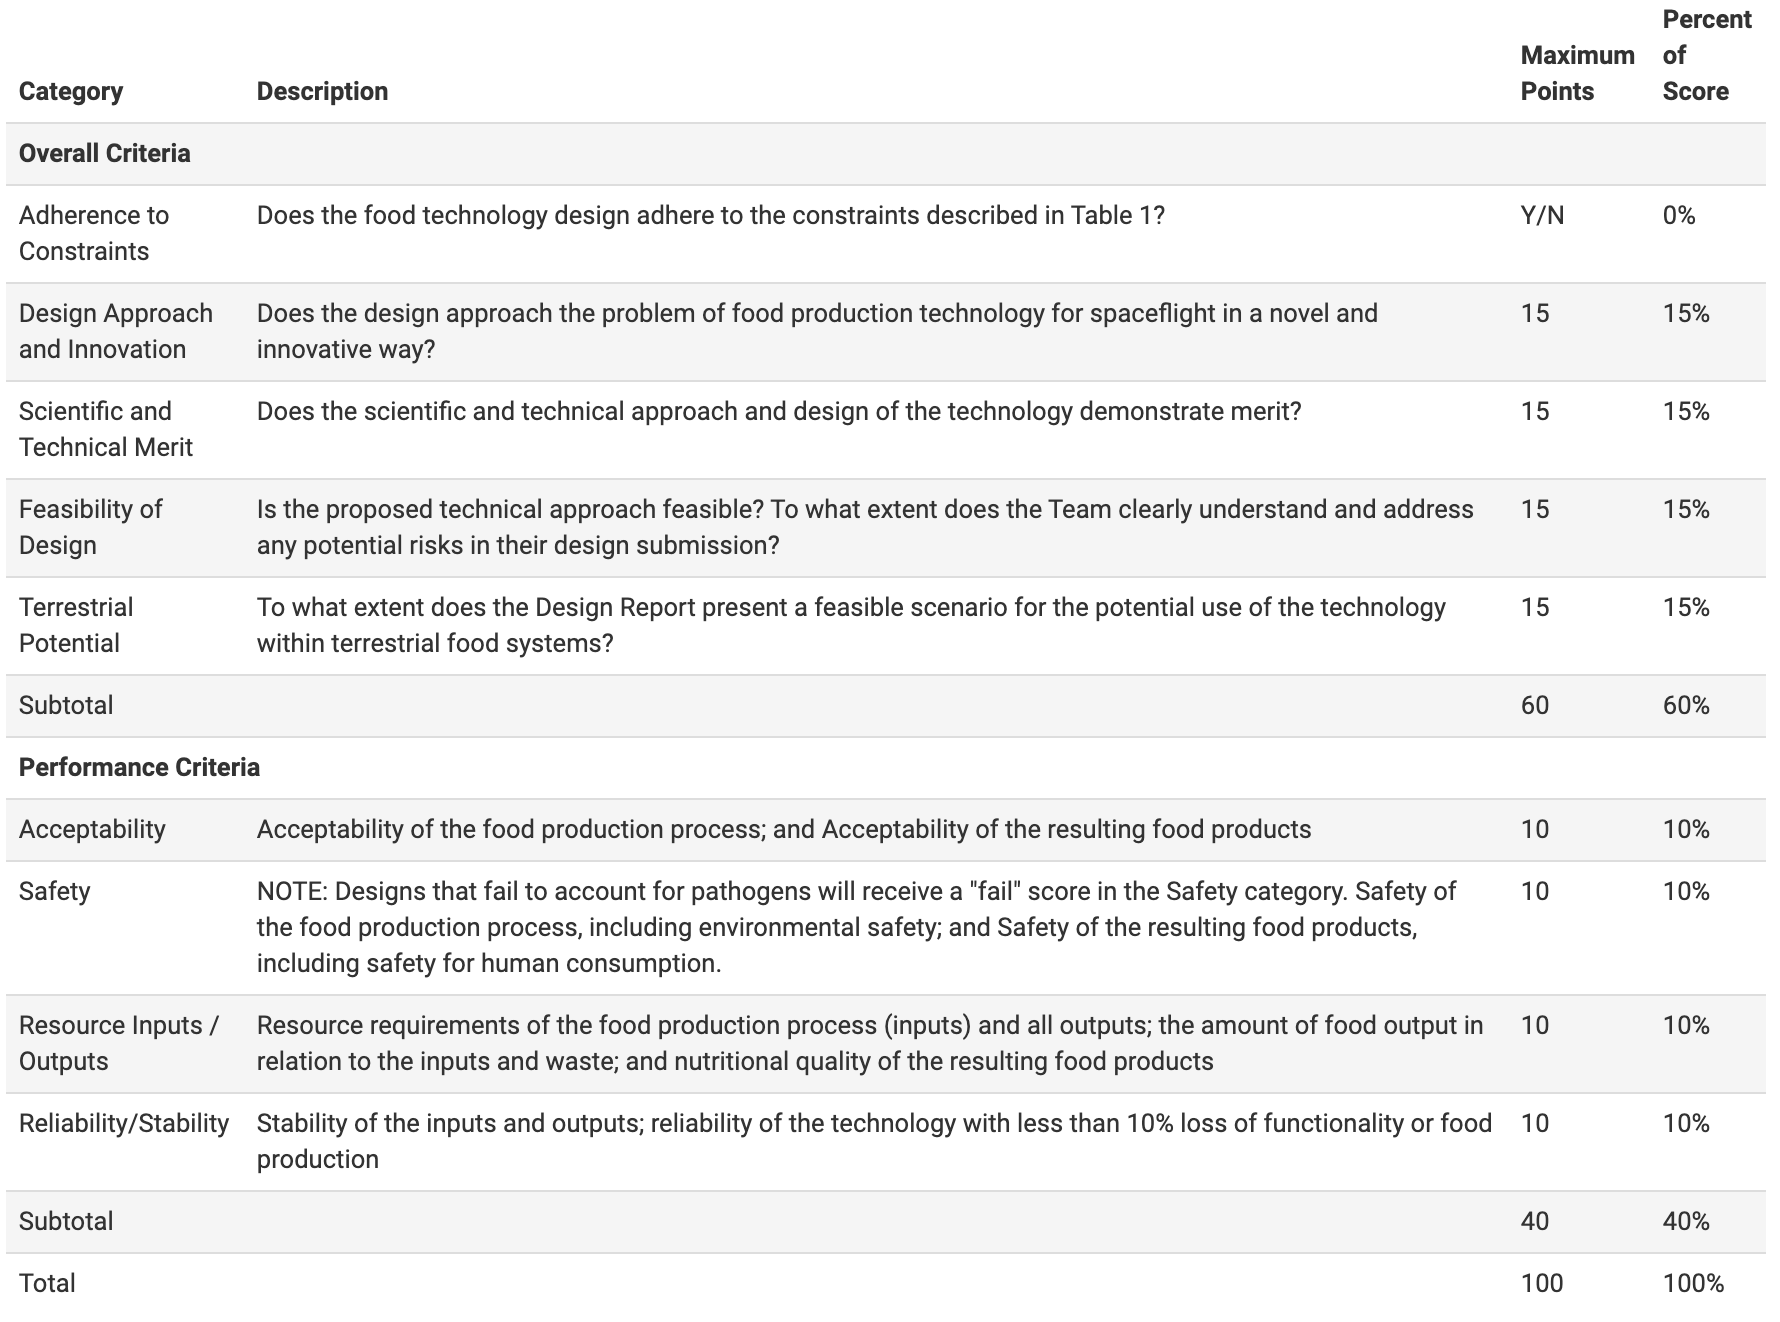
\includegraphics[width=15cm]{images/reportassessment.png}
    \hfill
    \caption{Design report assessment categories and weights \cite{applicantguide}.}
\end{figure}

\subsection{Animation Assessment Criteria}
\label{sec:animassessment}

\begin{figure}[h]
    \centering
    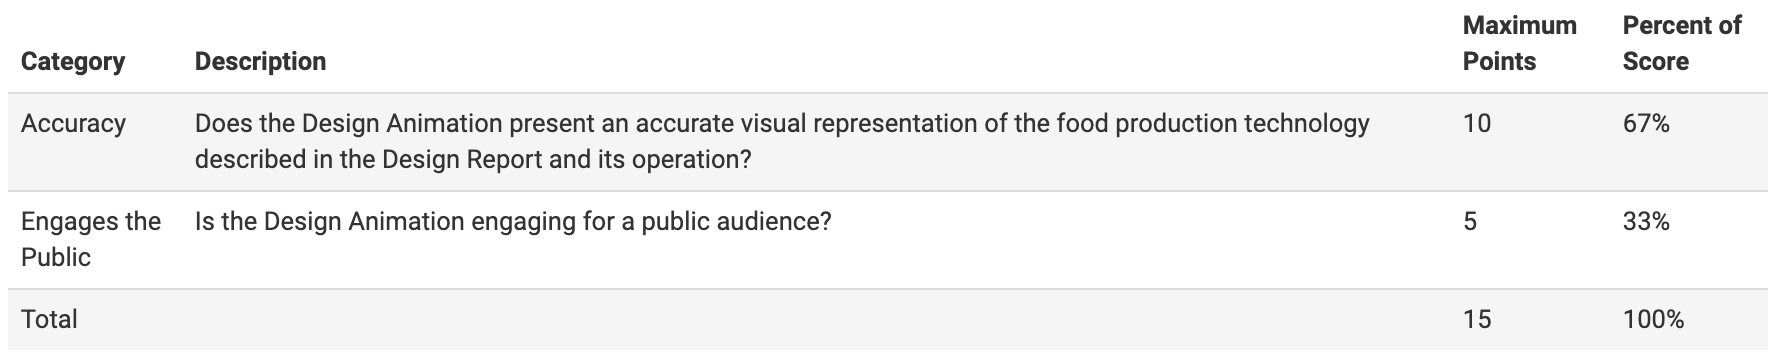
\includegraphics[width=15cm]{images/animassessment.png}
    \hfill
    \caption{Design animation assessment categories and weights \cite{applicantguide}.}
\end{figure}

\newpage

\section{Application Details}
\label{sec:application}

The contents of this appendix are adapted from \cite{applicantguide}, and should serve as the framework 
for developing the Phase 1 prototype.

A complete application package consists of the Challenge Application Form, with the following sections:

\begin{enumerate}
    \item Applicant details;
    \item Proposed solution details:
    \begin{enumerate}
        \item Design Abstract;
        \item Design Report (See Appendix \ref{sec:reportassessment});
        \item Design Animation (video; See Appendix \ref{sec:animassessment});
        \item Intellectual Property Details;
    \end{enumerate}
    \item Declaration;
    \item Survey (optional);
\end{enumerate}

\subsection{Design Abstract}



\end{appendices}

\newpage

\bibliographystyle{IEEEtran}

\bibliography{references}

\end{document}